\subsection{Réseau}

    \subsubsection{Transition du Lobby vers le jeu}
    
        Un système a été mis en place permettant le passage de la scène de lobby vers la scène de jeu.
        Ce système fonctionne a l'aide d'un timer, qui est synchronisé entre tout les joueurs, y compris ceux
        rejoignant le lobby après son lancement. La synchronisation se fait grâce à une fonctionnalité des salles Photon
        permettant de créer des propriétés spécifiques, couplé à la propriété PhotonNetwork.Time qui
        est identique pour tout les clients d'une salle au même moment, permettant une synchronisation
        "parfaite" des timers.
        Ce timer ne se lance uniquement après que le serveur soit à moitié remplit et dure 3 minutes. Si le nombre de joueurs descend en dessous de ce seuil, le timer s'arrête. De plus, qaund le serveur
        est complet, le temps d'attente est réduit à 30 secondes.
        A la fin du timer, le Master Client charge la map de jeu, qui est synchronisé avec tout les joueurs.


    \subsubsection{Synchronisation du lancement de partie}
        Une fois la transition effectué, il est nécessaire de synchroniser l'initialisation des différents composants
        permettant le fonctionnement d'une partie. Par exemple, il faut attendre que tout les joueurs finissent de charger
        la nouvelle scène avant d'instancier les joueurs sur la carte. Pour celà, un script s'occupe d'activer les différentes phases
        du lancement de partie suivant certaines conditions. Dans le cas de l'instantiation des joueurs, le script observe une propriété
        des joueurs déterminant si ces derniers ont chargés la map. Ainsi, le script de spawn des joueurs ne débute qu'une fois que tout les joueurs
        ont indiqué avoir chargé la carte.

    \subsubsection{Synchronisation des joueurs}
        Tout comme sur le lobby, les mouvements des joueurs ainsi que leurs animations sont synchronisés. Cependant,
        un deuxième élément s'ajoute à celà: l'apparition (spawn) des joueurs. Pour celà, des points d'apparitions (spawpoints)
        sont répartis sur la map. Le Master Client distribue ces points aux joueurs qui apparaîtront à l'endroit reçu. Celà permet
        de faire apparaîte chaque joueur à une position unique sur la carte : un point = un joueur, pas plus. Une fois celà fait,
        il faut également synhcroniser la réapparition des joueurs, pour celà on applique le même système, en ne prenant en compte que les joueurs
        morts.

    \subsubsection{Synchronisation de l'IA}

        La grande difficulté du système multijoueur est la synchronisation des PNJs. En effet, c'est une tâche important dû à la nature du jeu, 
        mais également difficile dû au grand nombre d'IA présentes sur la map.

        Tout d'abord, il faut synchroniser l'apparition des PNJs. Le Master Client instancie les personnages grâce à Photon ; ils sont donc au départ 
        placés et visibles de la même façon pour tout les joueurs.

        Tout d'abord, il faut synchroniser l'apparition des PNJs. Encore une fois, c'est le Master Client qui instancie les personnages
        grâce à Photon. Ils sont donc au départ placé de la même façon pour tout les joueurs. Il faut également synchroniser leur apparence.
        Encore une fois, cette dernière est déterminé par le Master Client puis partagé aux autres joueurs grâce à une méthode RPC.

        Mais les problèmes commencent au moment de synchroniser le mouvement des IA. Le système qui a été créé par Dov permet
        à l'IA de se déplacer sur la map, il faut maintenant que ce mouvement soit propagé de façon quasi-identique à tout les joueurs.
        Pour cela, plusieurs méthodes ont été envisagées:

            -L'utilisation de Photon Transform View, comme pour les joueurs. Ce système a vite montré ses limites, car inadapté à la synchronisation
            d'un grand nombre d'objets, fonctionant sur la base d'un envoi pseudo-continu d'informations. Ainsi de nombreux problèmes apparaissaient,
            et la synchronisation des mouvement en a souffert. 

            -Calcul de chemin client-side à partir du même point. L'idée est la suivante: le master client calcule un point, qui est la destination
            de l'IA, et la partage aux autres joueurs. Puis chaque joueur calcule le chemin pris par l'IA pour y arriver. Cela réduit considérablement la
            quantité d'information échangée, mais un autre problème se pose: le calcul de chemin pour les NavMesh Agents n'est pas déterministe. Ainsi le
            chemin calculé par chaque client à partir du même point n'est pas le même, ce qui entraîne également une désynchronisation de la position.

            -Enfin, le choix retenu est le calcul d'un chemin entier par le Master Client, qui envoie ensuite l'intégralité de ce chemin aux autres joueurs.
            Ainsi le chemin est le même pour tout le monde, mais l'envoi des points se fait de façon discrète: on envoit uniquement l'array de positions généré
            par le Master Client. Ce système permet d'avoir une synchronisation satisfaisante des déplacement et une utilisation minime de la bande passante.

        De plus, une fois le premier chemin créé et partagé aux joueurs de la salle, il est nécessaire d'activer le mouvement des PNJ de façon la plus simultanée possible.
        Le processus est le même que celui permettant de synchroniser les timers : on crée une propriété de la salle qui indique le moment exact où
        les IAs sont activés, une fonctionnalité de Photon permettant l'accés à une valeur identique sur tout les clients au même instant (PhotonNetwork.Time).

    \subsubsection{Synchronisation des assassinats et des morts}

        Une dernière partie de la synchronisation inclue celle des évènement de mort, pour les joueurs ainsi
        que les IA. Pour cela, il a été décidé d'utiliser le sytème d'Event Photon. Auparavant, la synchronisation de méthodes
        passait par l'utilisation de Photon View et de RPC. Mais le système de kill/death demande une propagation plus importante
        de l'évènement, car plusieurs systèmes différents doivent y réagir. C'est là que Photon rentre en jeu.

        En effet, ce dernier permet de synchroniser le déclenchement d'évènements. Pour cela, on utilise la méthode RaiseEvent ainsi
        qu'un code représentant notre évènement. Cette action appelle la méthode callback OnEvent, dans laquel il suffit d'associer le
        code de l'évènement à une méthode. Ainsi, à la mort d'un joueur, le tueur déclenche l'évènement mort en indiquant l'identité du
        joueur tué. Chaque joueur reçoit cet évènement et peut déterminer, par exemple, si le joueur mort est lui-même, ou bien si un
        autre joueur a tué sa cible... En bref, chaque client prend une décision en fonction de l'information reçue.
        Les détails du système de morts sont dans la partie gameplay.

        Une dernière partie de la synchronisation inclue celle des évènement de mort, pour les joueurs ainsi
        que les IA. Pour celà, il a été décidé d'utiliser le sytème d'Event Photon. Auparavant, la synchronisation de méthodes
        passait par l'utilisation de Photon View et de RPC. Mais le système de kill/death demande une propagation plus importante
        de l'évènement, car plusieurs systèmes différents doivent y réagir. C'est la que Photon rentre en jeu.

        En effet, ce dernier permet de synchroniser le déclenchement d'évènement. Pour celà, on utilise la méthode RaiseEvent ainsi
        qu'un code représentant notre évènement. Cette action appelle la méthode callback OnEvent, dans laquel il suffit d'associer le
        code de l'évènement à une méthode. Ainsi, à la mort d'un joueur, le tueur déclenche l'évènement mort en indiquant l'identité du
        joueur tué. Chaque joueur reçoit cette évènement et peut déterminer, par exemple, si le joueur mort est lui-même, ou bien si un
        autre joueur a tué sa cible... En bref, chaque client prend une décision en fonction de l'information reçu
        Les détails du système de morts sont dans la partie gameplay.

    \subsubsection{Synchronisation du déroulé de partie}
        De la même manière, un système d'event a été mis en place permettant de synchroniser les différentes étapes du jeu.

    \subsubsection{Chat photon}
	Enfin, un chat a été implémenté grâce à une librairie de Photon. Ce chat permet aux joueurs 
	d'une salle de communiquer entre eux, dans le lobby et en jeu.

	\begin{figure}[hbt!]
		\centering
		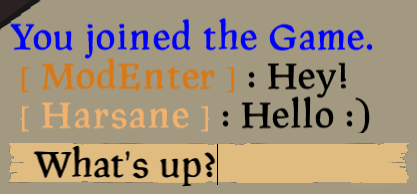
\includegraphics[scale=1]{chat.png}
		\caption{Démonstration du chat Photon}
	\end{figure}


